\chapter{Optimizing the Metric}
\label{sec:beta}

In a similar fashion as described in section \ref{chapter:alphalinkage}, this sections aims to find an optimized feature representation that is a linear combination of several metrics. For instance, images can have a 2-dimensional pixel representation and a text describing each image. Combining these features for clustering tasks can be problematic as it is not trivial how the optimal weight between these features should be. Does a word describe more than a fragment of the image, are the features equally important or does the pixel image lead to better clusterings? With $\beta$-linkage, we provide a framework based on $\alpha$-linkage that calculates different merges based on linear combinations of representations and leads to optimized clusterings.

\begin{figure}[h]
    \centering
    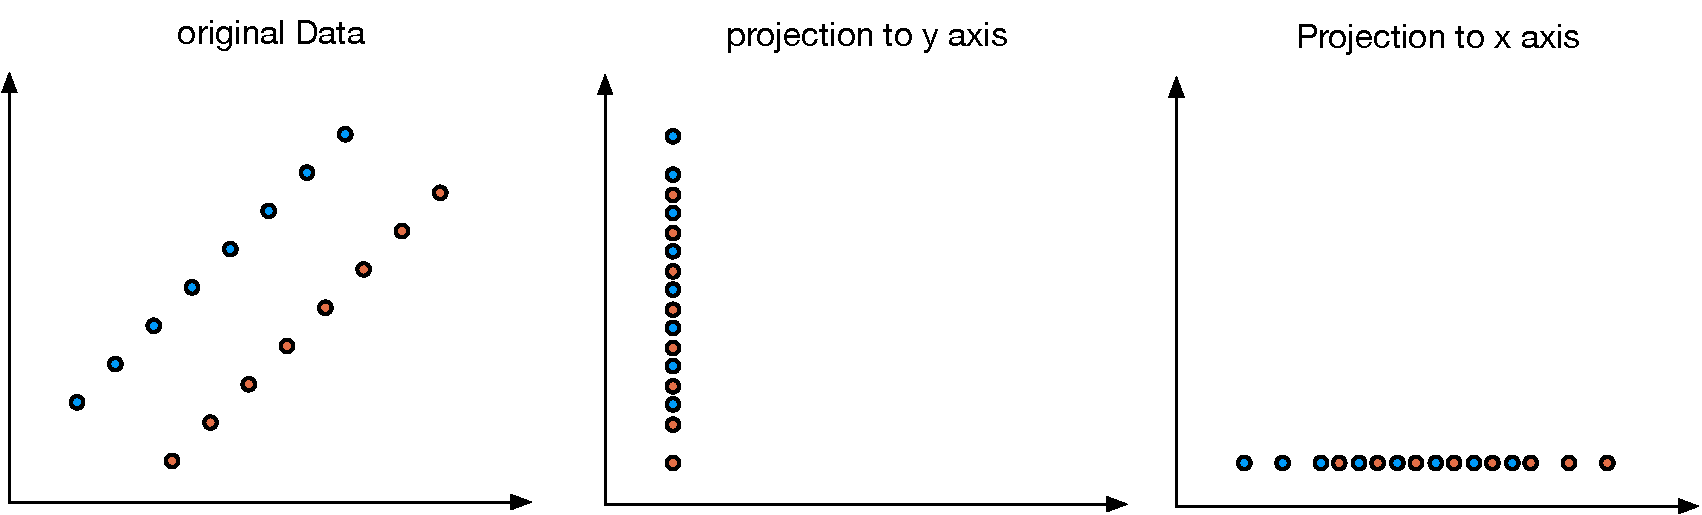
\includegraphics[width=0.7\textwidth]{images/ExampleDataset}
    \caption{Combining several metrics seems often natural and can lead to improved results as in this example where we project a dataset on the $x_1$- and the $x_2$-axis.}
    \label{fig:metrics}
\end{figure}

For instance, figure \ref{fig:metrics} shows a set of points that might be put in clusters easily. However, if you only look at the distance regarding the $x_1$-axis or the $x_2$-axis, a perfect clustering will no longer be possible, because each of the axes does not describe the spatial correlation anymore. This example is selected on purpose to motivate the following experiments where we learn optimal combinations of different metrics.\\ 

To interpolate between $d_0$ and $d_1$, we use the same interpolation as discussed in section \ref{chapter:alphalinkage}. We use a parameter $\beta \in [0,1]$ and weight the metrics as shown below.

\begin{align}
d_\beta(x,x') &= (1 - \beta) \cdot d_0(x,x') + \beta \cdot d_1(x,x') \nonumber \\
&= d_0(x,x') + \beta \cdot (d_1(x,x') - d_0(x,x'))
\label{eq:betalinkage}
\end{align}

We then compute all possible discontinuities by comparing the distances of given clusters $(x, x')$ and $(y, y')$. As $d_\beta(x,x')$ is a linear function depending on $\beta$ (see equation \ref{eq:betalinkage}), we can compute all discontinuities by solving the following equation.

\begin{equation*}
    \begin{aligned}
      \begin{gathered}
        d_\beta(x,x') = d_\beta(y,y')\\
        (1 - \beta) \cdot d_0(x,x') + \beta \cdot d_1(x,x') = (1 - \beta) \cdot d_0(y,y') + \beta \cdot d_1(y,y')\\
        d_0(x,x') - \beta \cdot d_0(x,x') + \beta \cdot d_1(x,x') = d_0(y,y') - \beta \cdot d_0(y,y') + \beta \cdot d_1(y,y')\\
        \beta \cdot (- d_0(x,x') + d_1(x,x') + d_0(y,y') - d_1(y,y')) = - d_0(x,x') + d_0(y,y')\\
        \beta = \frac{- d_0(x,x') + d_0(y,y')}{- d_0(x,x') + d_1(x,x') + d_0(y,y') - d_1(y,y')}
        \label{eq:discont}
      \end{gathered}
    \end{aligned}
\end{equation*}
As we know that the function $d_\beta$ is a linear function depending on $\beta$ and we showed that all discontinuities depend on four points, we know that there are at most $O(n^4)$ well-defined intervals $\mathcal{I}_i \in [0,1]$ for any clustering instance $S$, i.e. in any interval $\mathcal{I}_i$ the algorithm will merge the same two points. In order to efficiently calculate and evaluate all resulting cluster trees, we use an algorithm similar to algorithm \ref{alg:alphalinkage4} but adapted to $\beta$-linkage.

\begin{algorithm}
\textbf{Input:} Metrics $\dZero$ and $\dOne$, parameter $\beta \in [0,1]$, and clustering instance $S = \{x_1, \dots, x_n\}$.
\begin{enumerate}[nosep, leftmargin=*]
\item Let $\mathcal{N} = \{\leaf(x_1), \dots, \leaf(x_n)\}$ be the initial set of nodes (one leaf per point).
\item While $|\mathcal{N}| > 1$
\begin{enumerate}[nosep, leftmargin=*]
  \item Let $A, B \in \mathcal{N}$ be the clusters in $\mathcal{N}$ minimizing $\max_{a \in A, b \in B} \dbeta(a, b)$.
  \item Remove nodes $A$ and $B$ from $\mathcal{N}$ and add $\node(A,B)$ to $\mathcal{N}$.
\end{enumerate}
\item Return the cluster tree (the only element of $\mathcal{N}$).
\end{enumerate}
\caption{$\beta$-linkage Clustering}
\label{alg:betalinkage}
\end{algorithm}

A slight adaption that we need is to normalize the features such that for $\beta = 0.5$ we equally weight both distance matrices. We achieve this by dividing the features $f_1, \dots, f_k$ through the maximum value $f_{max}$. In this way, we scale the features into $[0,1]$ and do not lose the proportions as it would happen when e.g.\ using a min-max-scaler.